
%\clearpage

\section{Appendix}


%%%%%%%%%%%%%%%%%%%%%%%%%%%
%     _      __        _   
%  __| |___ / _|___ __| |_ 
% / _` / -_)  _/ -_) _|  _|
% \__,_\___|_| \___\__|\__|
%                          
%%%%%%%%%%%%%%%%%%%%%%%%%%%


\subsection{Defect} \label{appendix:defect}

Call the \textit{defect} a function $\lambda _ d : \mathbb{N}^d \mapsto \mathbb{N}$:

$$
\begin{array}{l}
\lambda _ 2 (|\alpha|,|\beta|) = \frac{ |\alpha| \cdot |\beta| }{ \text{min}(|\alpha|,|\beta|)^2 } \\
\lambda _ 3 (|\alpha|,|\beta|,|\gamma|) = \frac{ |\alpha| \cdot |\beta| \cdot |\gamma| }{ \text{min}(|\alpha|,|\beta|,|\gamma|)^3 }
\end{array}
$$

If there is a disjoint subdivision of a volume $V_0$ to $V_1  = ( V _ {0,0}, V _ {0,1}, \dots, V _ {0,m-1} )$,
$V _ 0  = \cup _ {k} V _ {0,k}$,
define the \textit{average defect} of the subdivided volume to be:

$$
\begin{array}{l}
  \lambda _ {s} ( V _ 1 ) = \sum _ {k} \frac{ \text{Vol}(V _ {0,k}) }{ \text{Vol}( V _ 0 ) } \cdot \lambda( V _ {0,k} )
\end{array}
$$

This weights the defect of each subdivided cuboid by its proportional volume.

The defect gives us a coarse idea of how lopsided or \textit{eccentric} a cuboid region is.
If the defect is too high, we might want to split the larger sides while keeping the smaller sides the same size.

Reducing the average defect attempts to make each subdivided cuboid more cube-like.
When subdivided cuboids are more cube-like, we say that the subdivided regions are more \textit{harmonious}.
The same idea is applied for 2D rectangles and rectangular regions that are more square like are said to be
more harmonious.

%%%%%%%%%%%%
%  ___    _ 
% |_  )__| |
%  / // _` |
% /___\__,_|
%           
%%%%%%%%%%%%

\subsection{2D Eccentric Split Threshold} \label{appendix:eccentric_2d}

\begin{figure}[h]
  \centering
  \includegraphics[width=\linewidth]{gilbert2d_eccentric_appendix.pdf}
  \caption{ When the length of the width-like dimension ($|\alpha|$) gets larger than a threshold of the height-like
            dimension ($\sigma |\beta|$), then the width like dimension is split into two. }
  \label{fig:eccentric_2d}
\end{figure}


In this section, we justify splitting the rectangle into
two roughly equal parts when $(|\alpha|/|\beta| > 3/2)$.

For the 2D Gilbert curve,
if the $\alpha$ side length is significantly longer than the $\beta$ side length,
we want to subdivide the rectangle into two nearly equal regions and recursively find
a Gilbert curve in each region.
We will justify the constant $(3/2)$ as the ratio threshold to split on using an argument
originally developed by L. Tautenhahn \footnote{ Given to us through personal communication with L. Tautenhahn }.

The defect of a rectangle of side length $|\alpha|$ and $|\beta|$ is, with $|\alpha| > |\beta|$:

$$
\begin{array}{ll}
  \lambda_2(|\alpha|, |\beta|) & = |\alpha| \cdot |\beta| / |\beta|^2 \\
   & = |\alpha| / |\beta|
\end{array}
$$

After a subdivision, if we assume $|\alpha| < 2 |\beta|$, the defect is:

$$
\begin{array}{ll}
  \lambda_2(|\alpha|/2, |\beta|) & = \frac{|\alpha|}{2} \cdot |\beta| / (\frac{|\alpha|}{2})^2 \\
   & = 2 |\beta| / |\alpha|
\end{array}
$$

We're looking for the condition when there's a defect reduction, so

$$
\begin{array}{ll}
    & \lambda_2(|\alpha|/2, |\beta|)  < \lambda_2(|\alpha|, |\beta|) \\
\to & 2 |\beta| / |\alpha| < |\alpha| / |\beta| \\
  \to & \sqrt{2} < |\alpha| / |\beta| \\
\end{array}
$$

Since $\sqrt{2} \approx 1.4142 < (3/2)$, if we choose $|\alpha| / |\beta| > (3/2)$ we can
be assured a defect reduction.

In the case when $|\alpha| > 2 |\beta|$, it is easy to verify that the defect is always reduced
\footnote{ The ratio of the defects before and after the split is $(1/2)$ }.

%%%%%%%%%%%%%%%%%%%%%%%%%%%%%%%%%%
%                    _       _    
%  ___ __ __ ___ _ _| |_ _ _(_)__ 
% / -_) _/ _/ -_) ' \  _| '_| / _|
% \___\__\__\___|_||_\__|_| |_\__|
%                                 
%%%%%%%%%%%%%%%%%%%%%%%%%%%%%%%%%%

\subsection{3D Eccentric Split Threshold}

Calculations in this section will justify the choice of threshold values for when to choose an eccentric $S$-split over a $J$-split.
Our concern is to find a simple ratio of when each of $\alpha$, $\beta$ or $\gamma$ are considered
"small enough" or "large enough", relative to the other lengths, to split on.

An enumeration of what conditions lead to an eccentric split are as follows:

$$
\begin{array}{ll}
  (1) & |\alpha| >> |\beta| \sim |\gamma| \\
  (2) & |\beta| >> |\alpha| \sim |\gamma| \\
  (3) & |\gamma| >> |\alpha| \sim |\beta| \\
  (4) & |\beta| << |\alpha| \sim |\gamma| \\
  (5) & |\alpha| << |\beta| \sim |\gamma| \\
  (6) & |\gamma| << |\alpha| \sim |\beta| \\
\end{array}
$$

A representation of the eccentric splits are enumerated in Figure \ref{fig:gilbert3DEccentricCase}.
The eccentric $S$-split split differs from the $J$-split as it's only partitioning the cuboid along
one or two dimensions instead of three.

For each of the six cases, we want to know what relative difference in sizes should be used
to determine when an eccentric split should be used and how to subdivide the cuboids so as to make
the resulting subdivided regions more cube-like or \textit{harmonious}.

Specifically, we want to find the ratio, $\sigma$, of when one dimension differs significantly from the others.
Further, we choose the ratio, $\rho$, of where to choose the first subdivision.
For the 2D case, choosing $\rho = \frac{1}{2}$ worked to make the resulting subdivided regions more harmonious.
We will need a different value of $\rho$ for most of the 3d cases to ensure a harmonious resulting subdivision.

In what follows, our goal is to choose a subdivision that will reduce the average defect.
We assume that the start and end of the path lie in the $\alpha$ dimension.

Since the start and end path lie on the $\alpha$ dimension, we are forced to split in the $\alpha$ axis
to subdivide the cuboid.

The chosen constants $\sigma$ and $\rho$ for each of the eccentric splits are not chosen optimally
to reduce average defect.
We chose $\sigma$ and $\rho$ as a compromise between providing simple ratios while
still providing a more harmonious subdivision.


%%%%%%%%%%%%%%%%%%%%%%%%%%%%%%%%%%
%        __     __          ____
%  ___ _/ /__  / /  ___ _   \ \ \
% / _ `/ / _ \/ _ \/ _ `/    > > >
% \_,_/_/ .__/_//_/\_,_/    /_/_/
%      /_/
%%%%%%%%%%%%%%%%%%%%%%%%%%%%%%%%%%

\subsection{$|\alpha| >> |\beta| \sim |\gamma|$}

\begin{figure}[h]
  \centering
  \includegraphics[width=\linewidth]{gilbert3d_eccentric_appendix_s0.pdf}
  \caption{ An $S_0$ eccentric subdivision showing the threshold, $\sigma$, used to determine when we should use this split. }
  \label{fig:eccentric_s0}
\end{figure}


\begin{itemize}
  \item $\sigma = \frac{5}{3}$
  \item $\rho = \text{n/a}$
  \item $|\alpha| > \sigma \cdot \text{min}( |\beta|, |\gamma|)$
  \item Shape template: $S_0$
\end{itemize}


We're splitting at the halfway point on $|\alpha|$ and we want to figure out
what the eccentric threshold is to split on.

Assume:

$$
\begin{array}{ll}
  s & = \text{min}(|\beta|, |\gamma|) \\
  \mu s & = \text{max}(|\beta|, |\gamma|) \\
  |\alpha| & = \sigma' s > \sigma s \\
  %& \sigma' > \sigma \ge \mu \ge 1 \\
\end{array}
$$

Call $\lambda_0$ the average defect of the original cuboid region and $\lambda_1$ the average defect
after the subdivision at the $\alpha$ halfway point:

$$
\begin{array}{ll}
  \lambda_0 & = \frac{ |\alpha| \mu s^2 }{ s^3 } = |\alpha| \mu / s \\
  \lambda_1 & = \left\{
    \begin{array}{lr}
      \frac{ (|\alpha| / 2) \mu s^3 }{ s^3 } = |\alpha| \mu / 2 & ( |\alpha| > 2 s) \\
      \frac{ (|\alpha| / 2) \mu s^3 }{ (|\alpha|/2)^3 } = 4 \mu s^2 / |\alpha|^2  & ( 2 s > |\alpha| > s)
    \end{array}
    \right. \\
  \lambda_1 / \lambda_0 & = \left\{
    \begin{array}{lr}
      1/2  & ( |\alpha| > 2 s) \\
      4 s^3 / |\alpha|^3 & ( 2 s > |\alpha| > s)
    \end{array}
    \right.
\end{array}
$$

We measure the relative defect reduction by the ratio $(\lambda_1 / \lambda_0)$.
For $|\alpha| > 2s$, $(\lambda_1 / \lambda_0 = 1/2)$, a defect reduction.

When $(2s > |\alpha| > s)$, set $|\alpha| = \sigma' \text{min}(|\beta|, |\gamma|)$.
We consider what values of $\sigma'$ will lead
to a defect reduction $(\lambda_1 / \lambda_0 < 1)$:

$$
\begin{array}{ll}
  \lambda_1 / \lambda_0 & = 4 s^3 / |\alpha|^3 < 1 \\
  \to & |\alpha|^3 > 4 s^3  \\
  \to & |\alpha| > 4^{\frac{1}{3}} s \\
  \to & \sigma' s > 4^{\frac{1}{3}} s \\
  \to & \sigma' > 4^{\frac{1}{3}} \\
\end{array}
$$

For any $\sigma > 4^{\frac{1}{3}}$, we know the average defect will be reduced.
For algorithmic simplicity, we've chosen the simple fraction $\sigma = \frac{5}{3}$ (as $\frac{5}{3} > 4^{\frac{1}{3}}$)
for the eccentric $S_0$ split ratio.



%%%%%%%%%%%%%%%%%%%%%%%%%%%%%%%%%%%%%%%%
%                                 ____  
%   ___ ____ ___ _  __ _  ___ _   \ \ \ 
%  / _ `/ _ `/  ' \/  ' \/ _ `/    > > >
%  \_, /\_,_/_/_/_/_/_/_/\_,_/    /_/_/ 
% /___/                                 
%%%%%%%%%%%%%%%%%%%%%%%%%%%%%%%%%%%%%%%%


\subsection{ $|\gamma| >> |\alpha| \sim |\beta|$ }


\begin{figure}[h]
  \centering
  \includegraphics[width=\linewidth]{gilbert3d_eccentric_gamma_gt.pdf}
  \caption{ An $S_1$ eccentric subdivision showing the threshold, $\sigma$, used to determine when we should use this split
            and the split point ratio, $\rho$, to reduce the defect for a more harmonious subdivision. }
  \label{fig:eccentric_gamma_gt}
\end{figure}



%In what follows, we assume $\gamma$ is the elongated axis.
%After the calculation, we will discuss the case when $\beta$ is the shorter axis.

\begin{itemize}
  \item $\sigma = \frac{3}{2}$
  \item $\rho = \frac{1}{3}$
  \item $|\gamma| > \sigma \cdot \text{min}( |\alpha|, |\beta|)$
  \item Shape template: $S_1$
\end{itemize}


Define:

$$
\begin{array}{ll}
  s & = \text{min}(|\alpha|, |\beta|) \\
  \mu s & = \text{max}(|\alpha|, |\beta|) \\
  |\gamma| & = \sigma' s > \sigma s \\
   %& \sigma' > \sigma \ge \mu \ge 1 \\
\end{array}
$$

$\sigma$ represents our threshold value of when to choose the $S_1$ subdivision scheme.
If we've met the condition that $|\gamma| > \text{max}(|\alpha|, |\beta|) > \sigma \text{min}(|\alpha|, |\beta|)$,
we split at the $\rho$ point
along the $\gamma$ axis and split the remaining smaller base cuboid at the halfway point on the $\alpha$ axis.

Considering what combination of $\sigma$ and $\rho$ will lead to a defect reduction can be done
but we satisfy ourselves with showing that a choice of the simple fractions
$\sigma = 3/2$ and $\rho = 1/3$ suffices to ensure a defect reduction.

From the choice of $\sigma$ and $\rho$, we have that $(\rho \sigma \ge 1/2)$, ensuring that
the minimum side length of the smallest subdivided cuboid region is $(s/2)$ or $(\mu s/2)$.

As a technical addition, we introduce $\mu' = |\alpha| / s$, with  $\mu'$ equal to either $1$ or $\mu$
and $\mu' \ge 1$.

To show an average defect reduction, we
show $\lambda_1 < \lambda_0$ for our choice of $\sigma$ and $\rho$.

$$
\begin{array}{ll}
  \lambda_0 & = \frac{ |\gamma| \mu s^2 }{ s^3 } = |\gamma| \mu / s  \\
  \lambda_1 & = 2 (\frac{\rho}{2}) \left( \frac{(\frac{s}{2}) (\mu s) \rho |\gamma| }{(\frac{s}{2})^3 (\mu')^3 } \right)  
              + (1-\rho) \left( \frac{ (1-\rho) |\gamma| \mu s^2}{s^3} \right) \\
 & =  \frac{ 4 \rho^2 \mu |\gamma|}{s (\mu')^3} + \frac{(1-\rho)^2 \mu |\gamma|}{s}  \\
\end{array}
$$

$$
\begin{array}{llr}
 & \lambda_1 / \lambda_0 < 1 & \\
 \to & \left( \frac{ 4 \rho^2 \mu |\gamma|}{s (\mu')^3} + \frac{(1-\rho)^2 \mu |\gamma|}{s} \right) / \left( |\gamma|\mu / s \right)  < 1 & \\
 \to & (4 \rho^2 / (\mu')^3 ) + (1- \rho)^2 < 1 & \\
 \to & 4 \rho^2 + (1- \rho)^2 < 1 &  (\mu' > 1) \\
 \to & 5 \rho^2 + 1 - 2 \rho < 1 &  \\
 \to & \rho  < 2/5 &  (\rho \ne 0) \\
\end{array}
$$

For our choice of $\sigma = 3/2$, the average defect is reduced
so long as the $\gamma$ split point of $\rho < 2/5$.
We've chosen $\rho = 1/3 < 2/5$, ensuring an average defect reduction.

\subsection{ $|\beta| << |\alpha| \sim |\gamma|$ }

%%%%%%%%%%%%%%%%%%%%%%%%%%%%%
%    __       __         ____
%   / /  ___ / /____ _  / / /
%  / _ \/ -_) __/ _ `/ < < < 
% /_.__/\__/\__/\_,_/   \_\_\
%                            
%%%%%%%%%%%%%%%%%%%%%%%%%%%%%

\begin{figure}[h]
  \centering
  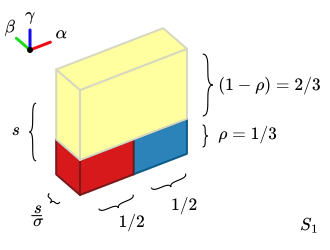
\includegraphics[width=\linewidth]{gilbert3d_eccentric_beta_lt.pdf}
  \caption{ An $S_1$ eccentric subdivision showing the threshold, $\sigma$, used to determine when we should use this split
            and the split point ratio, $\rho$, to reduce the defect for a more harmonious subdivision. }
  \label{fig:eccentric_beta_lt}
\end{figure}


\begin{itemize}
  \item $\sigma = \frac{3}{2}$
  \item $\rho = \frac{1}{3}$
  \item $|\beta| < \text{min}( |\alpha|, |\gamma|) / \sigma$
  \item Shape template: $S_1$
\end{itemize}



For the case when $|\beta|$ is much smaller than $|\alpha|$ and $|\gamma|$,
($|\beta| < \text{min}(|\alpha|, |\gamma|) / \sigma$),
we show that if we still use the same subdivision scheme, splitting $\gamma$ at the $\rho$ point and halfway for the
remainder cuboid on the $\alpha$, still leads to an average defect reduction.

Here, we take:

$$
\begin{array}{ll}
  s & = \text{min}(|\alpha|, |\gamma|) \\
  \mu s & = \text{max}(|\alpha|, |\gamma|) \\
  |\beta| & = s / \sigma' < s / \sigma \\
   %& \sigma' \ge \sigma > \mu \ge 1 \\
\end{array}
$$

Though the calculation is somewhat similar, there's an added complication that the minimum side length is
after the subdivision.
We add an extra term, $\omega$ to help with our calculation:

$$
\begin{array}{llr}
  \omega & = \text{min}( \frac{s}{2}, \rho s, |\beta| = \frac{s}{\sigma'} < \frac{s}{\sigma} ) & \\
   & = \text{min}( \rho s, |\beta| ) & (\rho = 1/3 < 1/2) \\
\end{array}
$$

Only taking terms with $\rho$ or $s$ as a factor since $\mu \ge 1$. 

We calculate the average defect reduction before and after the subdivision:


$$
\begin{array}{ll}
  \lambda_0 & = \frac{ |\beta| \mu s^2 }{ |\beta|^3 } = \mu s^2 / |\beta|^2  \\
  \lambda_1 & = 2 (\frac{\rho}{2}) \left( \frac{\mu (\frac{s}{2}) \rho s |\beta| }{\omega^3} \right)  
              + (1-\rho) \left( \frac{ (1-\rho) |\beta| \mu s^2}{ |\beta|^3} \right) \\
  & =  \frac{ \rho^2 \mu s^2 |\beta| }{2 \omega^3} + \frac{ (1-\rho)^2 \mu s^2 }{ |\beta|^2 } \\
\end{array}
$$

Suffice it to check that $\lambda_1 / \lambda_0 < 1$:

$$
\begin{array}{llr}
  \lambda_1 / \lambda_0 & = \frac{\rho^2 |\beta|^3}{2 \omega^3} + (1-\rho)^2 < 1 & \\
  \to & \frac{|\beta|}{\omega} < 10^{\frac{1}{3}} & (\rho = 1/3) \\
\end{array}
$$

$$
\begin{array}{ll}
  \frac{|\beta|}{\omega} & = \left\{
    \begin{array}{lr}
      1 < 10^{\frac{1}{3}} & (\omega = |\beta|) \\
      \frac{|\beta|}{\rho s} = \frac{1}{\rho \sigma'} < \frac{1}{\rho \sigma} = 1/2 < 10^{\frac{1}{3}}  & (\omega = \rho s = s / 3) \\
    \end{array}
  \right. \\
\end{array}
$$

Showing our choice of $\sigma = 3/2$ and $\rho = 1/3$ provides an average defect reduction even in the case
of $|\beta|$ small relative to the other two side lengths.



\subsection{$|\beta| >> |\alpha| \sim |\gamma|$}

%%%%%%%%%%%%%%%%%%%%%%%%%%%%%%%
%    __       __         ____  
%   / /  ___ / /____ _   \ \ \ 
%  / _ \/ -_) __/ _ `/    > > >
% /_.__/\__/\__/\_,_/    /_/_/ 
%%%%%%%%%%%%%%%%%%%%%%%%%%%%%%%

\begin{figure}[h]
  \centering
  \includegraphics[width=\linewidth]{gilbert3d_eccentric_beta_gt.pdf}
  \caption{ An $S_2$ eccentric subdivision showing the threshold, $\sigma$, used to determine when we should use this split
            and the split point ratio, $\rho$, to reduce the defect for a more harmonious subdivision. }
  \label{fig:eccentric_beta_gt}
\end{figure}

\begin{itemize}
  \item $\sigma = \frac{3}{2}$
  \item $\rho = \frac{1}{3}$
  \item $|\beta| > \sigma \cdot \text{min}( |\alpha|, |\gamma|)$
  \item Shape template: $S_2$
\end{itemize}

Here $|\beta|$ is the eccentric length, surpassing $\sigma = 3/2$ of the minimum
of the other two lengths to
trigger an $S_2$ subdivision.

To verify the constants chosen lead to an average defect reduction, define:

$$
\begin{array}{ll}
  s & = \text{min}(|\alpha|, |\gamma|) \\
  \mu s & = \text{max}(|\alpha|, |\gamma|) \\
  \mu' s & = |\alpha| \\
  \sigma' s & = |\beta| > \sigma s \\
  %& \sigma' \ge \sigma > \mu \ge 1 \\
\end{array}
$$

The average defect before the subdivision, $\lambda_0$, and after, $\lambda_1$:

$$
\begin{array}{ll}
  \lambda_0 & = \frac{|\beta| \mu s^2 }{s^3} = |\beta| \mu / s \\
  \lambda_1 & = \rho \left( \frac{ \rho |\beta| s (\frac{s}{2}) \mu }{ (\mu')^3 (\frac{s}{2})^3 } \right) +
    (1-\rho) \left( \frac{(1-\rho)|\beta| s^2 \mu}{s^3} \right) \\
    & = \frac{4 \sigma^2 |\beta| \mu}{(\mu')^3 s} + \frac{(1-\rho)^2 |\beta| \mu }{s} 
\end{array}
$$

Since $|\beta| > \sigma s$, $\text{min}( \rho |\beta| > \rho \sigma s > \frac{s}{2}, \frac{s}{2}) = \frac{s}{2}$
and $\text{min}( (1-\rho)|\beta| > (1-\rho)\sigma s = s, s) = s$, giving us the denominator of the
defect calculation above.

The average defect reduction ratio:

$$
\begin{array}{llr}
  \lambda_1 / \lambda_0 & = \frac{4 \rho^2}{(\mu')^3} + (1-\rho)^2 & \\
   & < 4 \rho^2 + (1-\rho)^2 & (\mu' \ge \mu \ge 1) \\
   & = 8/9 < 1 \\
\end{array}
$$

Showing an average defect reduction.

\subsection{ $|\alpha| << |\beta| \sim |\gamma|$ }

%%%%%%%%%%%%%%%%%%%%%%%%%%%%%%%%
%        __     __          ____
%  ___ _/ /__  / /  ___ _  / / /
% / _ `/ / _ \/ _ \/ _ `/ < < < 
% \_,_/_/ .__/_//_/\_,_/   \_\_\
%      /_/                      
%%%%%%%%%%%%%%%%%%%%%%%%%%%%%%%%

\begin{figure}[h]
  \centering
  \includegraphics[width=\linewidth]{gilbert3d_eccentric_alpha_lt.pdf}
  \caption{ An $S_1$ eccentric subdivision showing the threshold, $\sigma$, used to determine when we should use this split
            and the split point ratio, $\rho$, to reduce the defect for a more harmonious subdivision. }
  \label{fig:eccentric_alpha_lt}
\end{figure}


\begin{itemize}
  \item $\sigma = \frac{3}{2}$
  \item $\rho = \frac{1}{3}$
  \item $|\alpha| < \text{min}( |\beta|, |\gamma|) / \sigma$
  \item Shape template: $S_2$
\end{itemize}


Here $|\alpha|$ is the eccentric smaller length, falling below $1/\sigma = 2/3$
of the minimum of the other two lengths to trigger an $S_2$ subdivision.

To verify the constants chosen lead to an average defect reduction, define:

$$
\begin{array}{ll}
  s & = \text{min}(|\beta|, |\gamma|) \\
  \mu s & = \text{max}(|\beta|, |\gamma|) \\
  \sigma' s & = |\beta| > \sigma s \\
  \omega & = \text{min}( \rho s, \frac{|\alpha|}{2} = \frac{s}{2 \sigma'} < \frac{s}{2\sigma} = \frac{s}{3} ) \\
   & = |\alpha|/2 \\
  %& \sigma' \ge \sigma \ge \mu \ge 1 \\
\end{array}
$$

For convenience, we take $\omega$ to the smallest side length of the bottom subdivided region.

The average defect before the subdivision, $\lambda_0$, and after, $\lambda_1$:

$$
\begin{array}{ll}
  \lambda_0 & = \frac{ |\alpha| s^2 \mu }{ |\alpha|^3 } = \frac{\mu s^2}{|\alpha|^2} \\
  \lambda_1 & = \rho \left( \frac{ (|\alpha|/2) (\rho s) s \mu  }{ \omega^3 } \right)
    + (1-\rho) \left( \frac{ |\alpha| (1-\rho) s^2 \mu  }{ |\alpha|^3 } \right) \\
    & = \frac{ \rho^2 |\alpha| s^2 \mu }{ 2 (|\alpha|/2)^3 } + \frac{ (1-\rho)^2 s^2 \mu }{ |\alpha|^2 } \\
    & = \frac{ 4 \rho^2 s^2 \mu }{ |\alpha|^2 } + \frac{ (1-\rho)^2 s^2 \mu }{ |\alpha|^2 } \\
\end{array}
$$

The defect reduction:

$$
\begin{array}{ll}
  \lambda_1 / \lambda_0 & = 4 \rho^2 + (1-\rho)^2 \\
   & = 8/9 < 1 \\
\end{array}
$$

Confirming a defect reduction.

\subsection{ $|\gamma| << |\alpha| \sim |\beta|$ }

%%%%%%%%%%%%%%%%%%%%%%%%%%%%%%%%%%%%%%
%                                 ____
%   ___ ____ ___ _  __ _  ___ _  / / /
%  / _ `/ _ `/  ' \/  ' \/ _ `/ < < < 
%  \_, /\_,_/_/_/_/_/_/_/\_,_/   \_\_\
% /___/                               
%%%%%%%%%%%%%%%%%%%%%%%%%%%%%%%%%%%%%%

\begin{figure}[h]
  \centering
  \includegraphics[width=\linewidth]{gilbert3d_eccentric_gamma_lt.pdf}
  \caption{ An $S_1$ eccentric subdivision showing the threshold, $\sigma$, used to determine when we should use this split
            and the split point ratio, $\rho$, to reduce the defect for a more harmonious subdivision. }
  \label{fig:eccentric_gamma_lt}
\end{figure}


\begin{itemize}
  \item $\sigma = \frac{3}{2}$
  \item $\rho = \frac{1}{3}$
  \item $|\gamma| < \text{min}( |\alpha|, |\beta|) / \sigma$
  \item Shape template: $S_2$
\end{itemize}


Here $|\gamma|$ is the eccentric smaller length, falling below $1/\sigma = 2/3$
of the minimum of the other two lengths to trigger an $S_2$ subdivision.

To verify the constants chosen lead to an average defect reduction, define:

$$
\begin{array}{ll}
  s & = \text{min}(|\alpha|, |\beta|) \\
  \mu s & = \text{max}(|\alpha|, |\beta|) \\
  s / \sigma' & = |\gamma| < s / \sigma \\
  \omega & = \text{min}( |\gamma|, \rho s ) \\
  %& \sigma' \ge \sigma \ge \mu \ge 1 \\
\end{array}
$$

For convenience, we take $\omega$ to the smallest side length of the bottom subdivided region.

The average defect before the subdivision, $\lambda_0$, and after, $\lambda_1$:

$$
\begin{array}{ll}
  \lambda_0 & = \frac{ |\gamma| s^2 \mu }{ |\gamma|^3 } = \frac{\mu s^2}{|\gamma|^2} \\
  \lambda_1 & = \rho \left( \frac{ |\gamma| (\rho s) (s/2) \mu  }{ \omega^3 } \right)
    + (1-\rho) \left( \frac{ |\gamma| (1-\rho) s^2 \mu  }{ |\gamma|^3 } \right) \\
    & = \frac{ \rho^2 |\gamma| s^2 \mu }{ 2 \omega^3 } + \frac{ (1-\rho)^2 s^2 \mu }{ |\gamma|^2 } \\
\end{array}
$$

The defect reduction:

$$
\begin{array}{ll}
  \lambda_1 / \lambda_0 & = \frac{\rho^2 |\gamma|^3 }{ 2 \omega^3 }  + (1-\rho)^2 \\
  & = \left\{
      \begin{array}{lr}
        \frac{\rho^2}{2} + (1-\rho)^2 = 1/2 < 1 & (\omega = |\gamma|) \\
        \frac{ \rho^2 (\frac{s}{\sigma'})^3 }{ 2 (\frac{s}{3})^3 } + (1-\rho)^2 & (\omega = \frac{s}{3}, |\gamma| = \frac{s}{\sigma'}) \\
        = \frac{ \rho^2 3^3 }{ 2 (\sigma')^3 } + (1-\rho)^2 & \\
        \le \frac{ \rho^2 3^3 }{ 2 (\sigma)^3 } + (1-\rho)^2 & \\
         = \frac{ \rho^2 3^3 }{ 2 (3/2)^3 } + (1-\rho)^2 & \\
         = 4 \rho^2  + (1-\rho)^2  = 8 / 9 < 1 & \\
      \end{array}
    \right. \\
\end{array}
$$

Confirming a defect reduction.


